\documentclass[12pt]{amsart}
\usepackage{amsmath}
\usepackage{graphicx}

\newcommand{\me}{
    \author{Abhay Shankar K: cs21btech11001}
    \maketitle
}
\begin{document}
\title{Assignment 1}
\me

    \section*{Exercise 1}
    Output for : \begin{itemize}
        \item department
    
        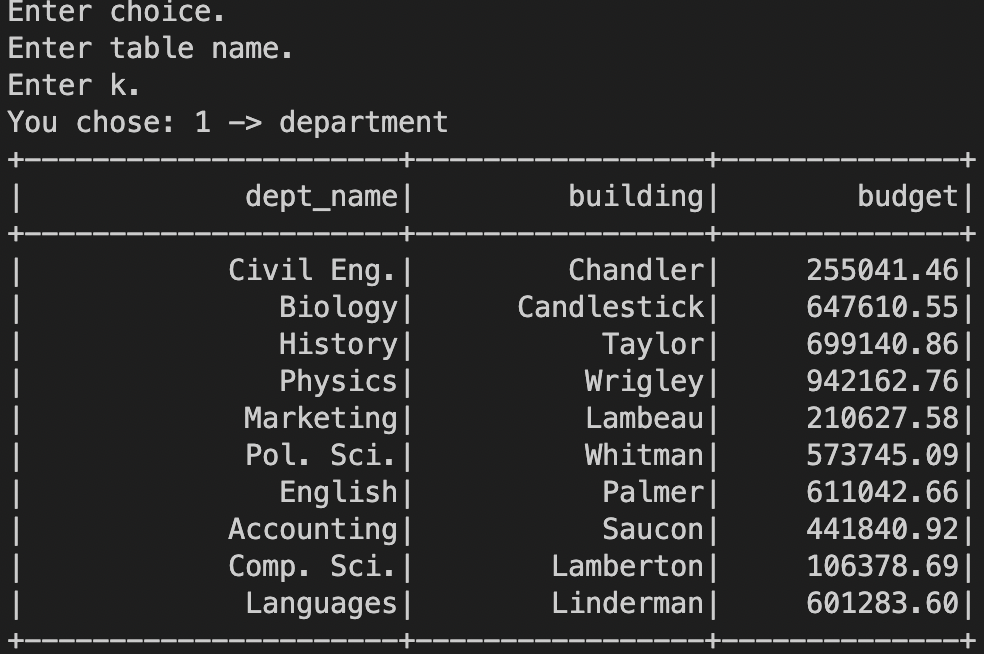
\includegraphics[scale = 0.5]{1_1.png}
    
        \item section 
    
        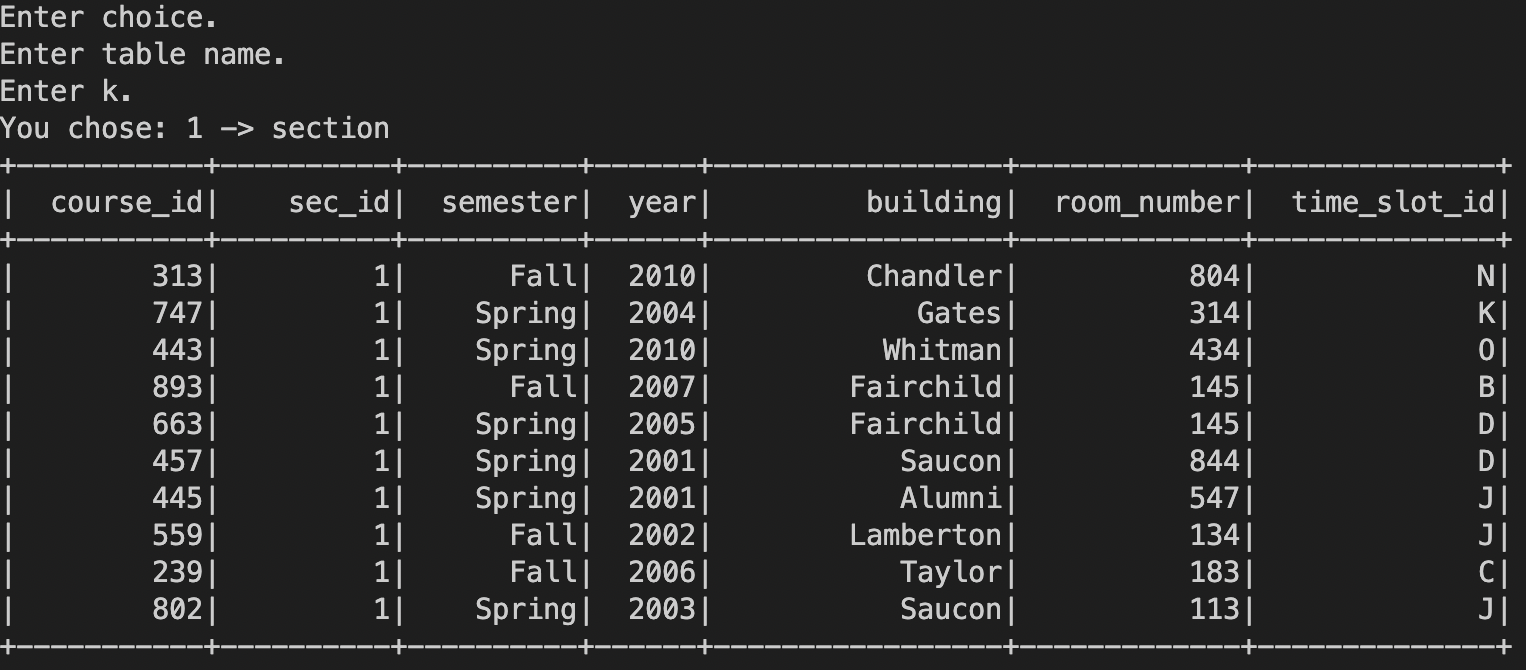
\includegraphics[scale = 0.5]{1_2.png}
    
        \item takes

        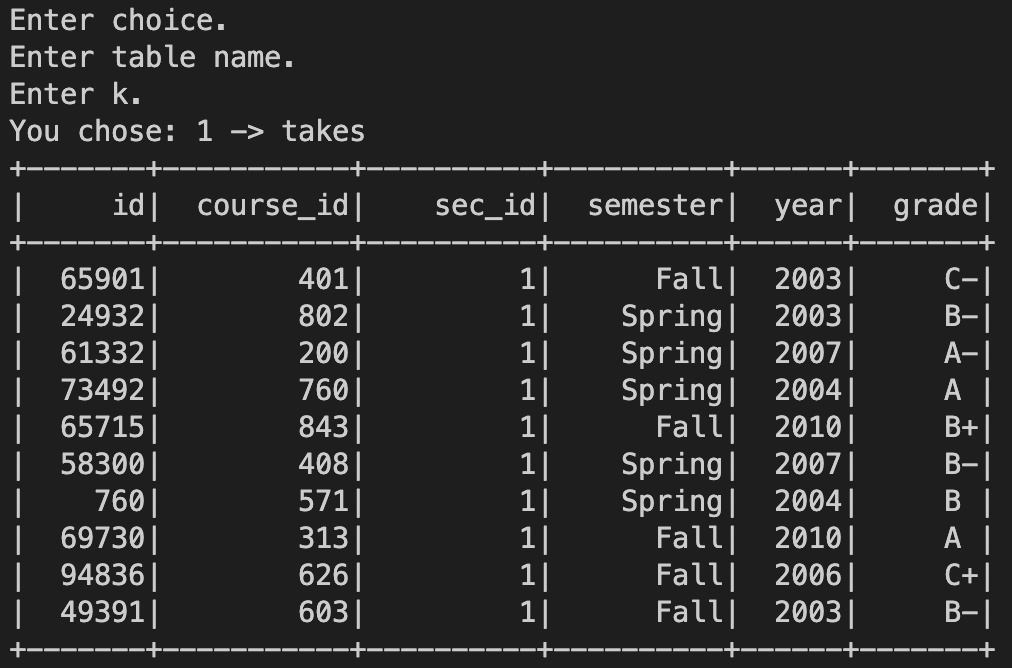
\includegraphics[scale = 0.5]{1_3.png}
    
    \end{itemize}
    
    
    
    
    \section*{Exercise 2}

    Output the course id and title of all the prerequisites for the following courses: 276, 647, 496

        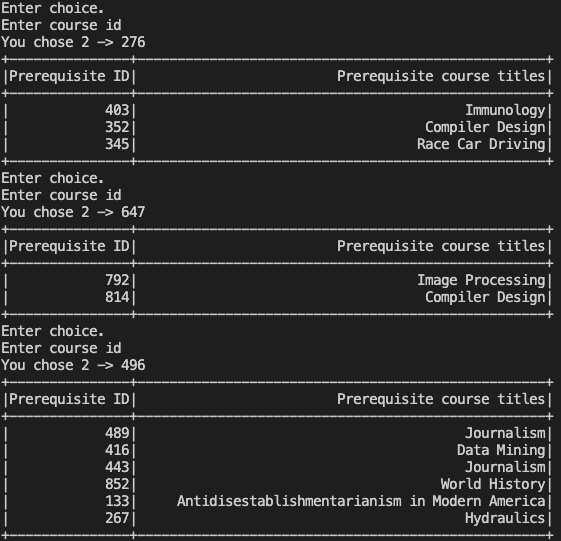
\includegraphics[scale = 0.5]{2.png}

    \section*{Exercise 3}

    Write any 5 varied test cases that you created to test the trigger. They should test different aspects of whether the trigger is working or not.

        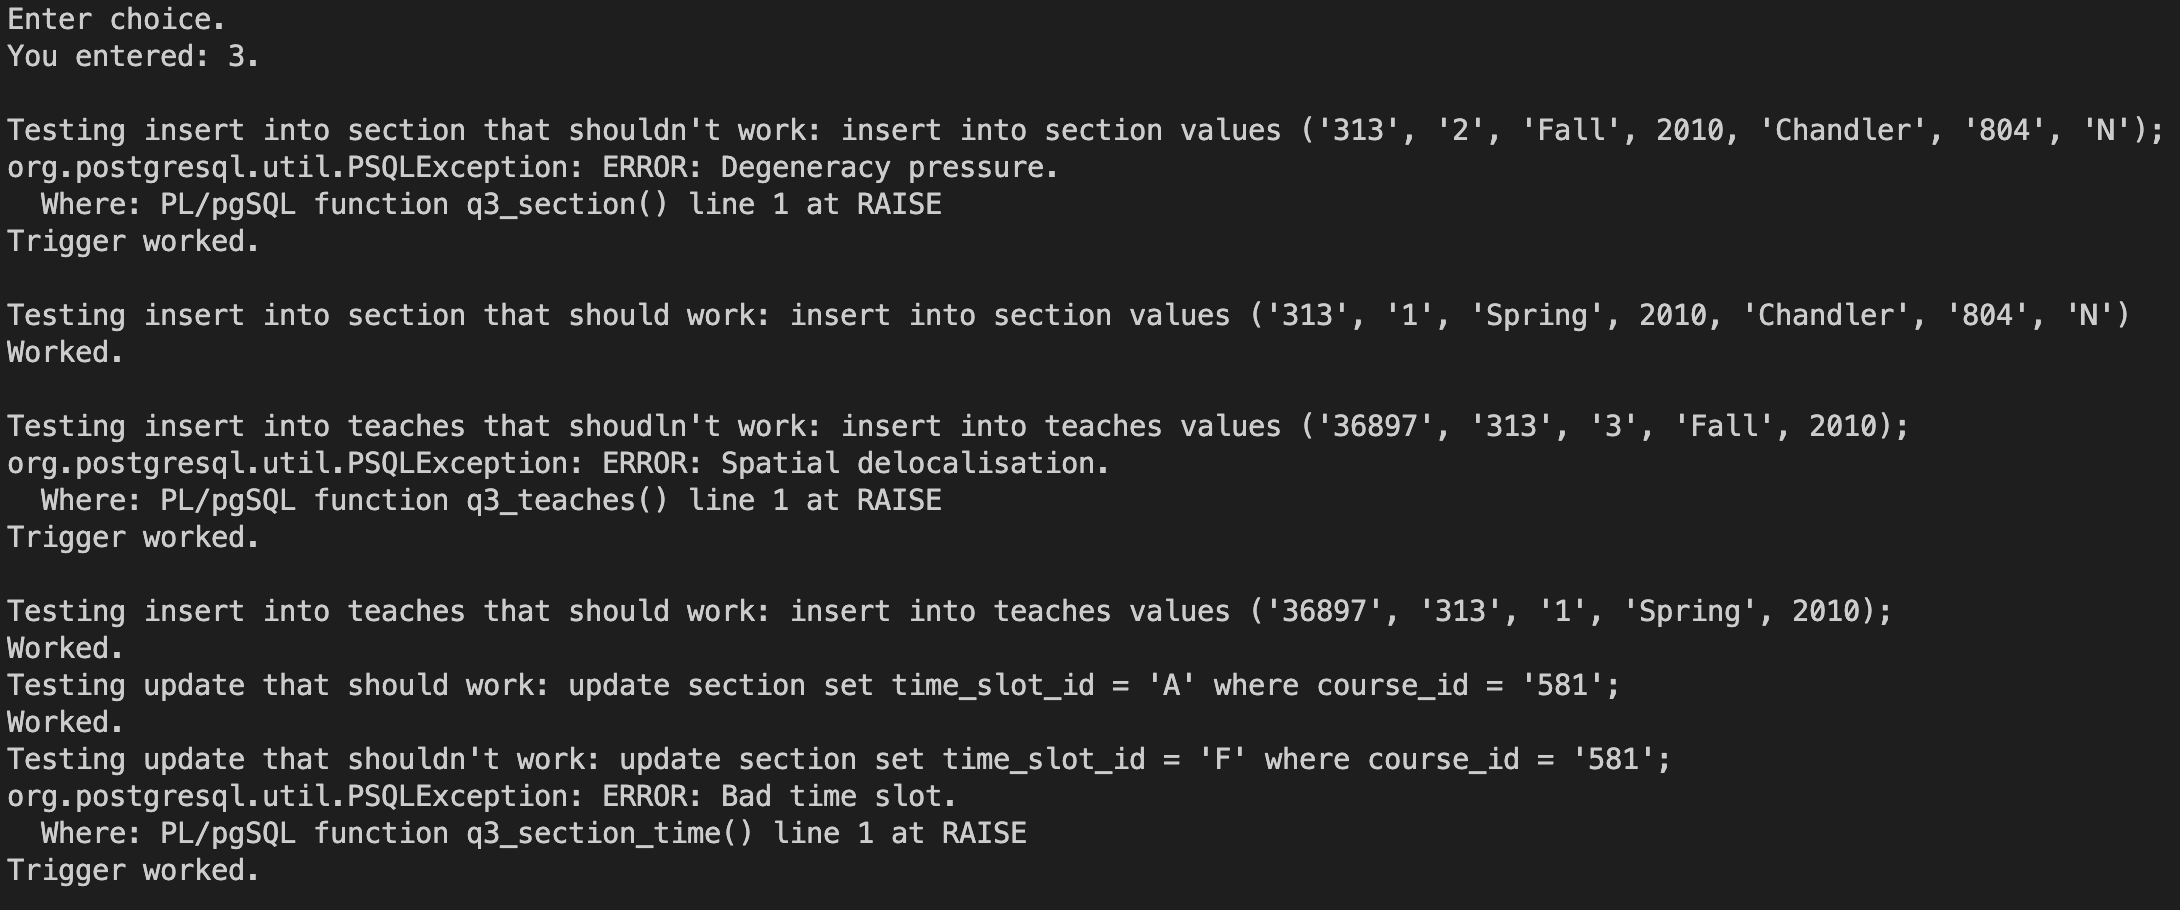
\includegraphics[scale = 0.35]{3.png}

        Here, the six test cases involve three tuples that would result in inconsistencies, two in section and one in teaches, each violating one trigger. Their outputs are shown, after an exception is raised by their respective triggers.
        The other three work, showing that each trigger allows insertion of valid tuples.
    
        \section*{Exercise 4}

    Print the CGPA for the following roll numbers: 76672, 90567, 4582, 81258

        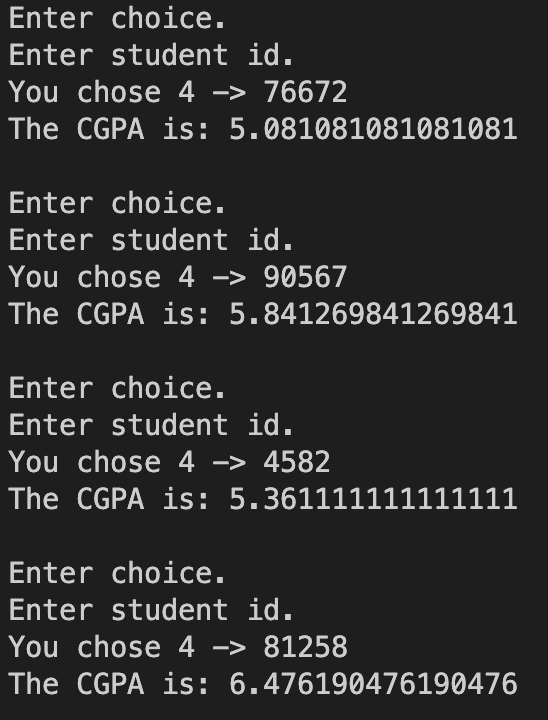
\includegraphics[scale = 0.5]{4.png}
\newpage
    \section*{Exercise 5}

    Subquestion 1: Print the top-5 students in terms of CGPA


    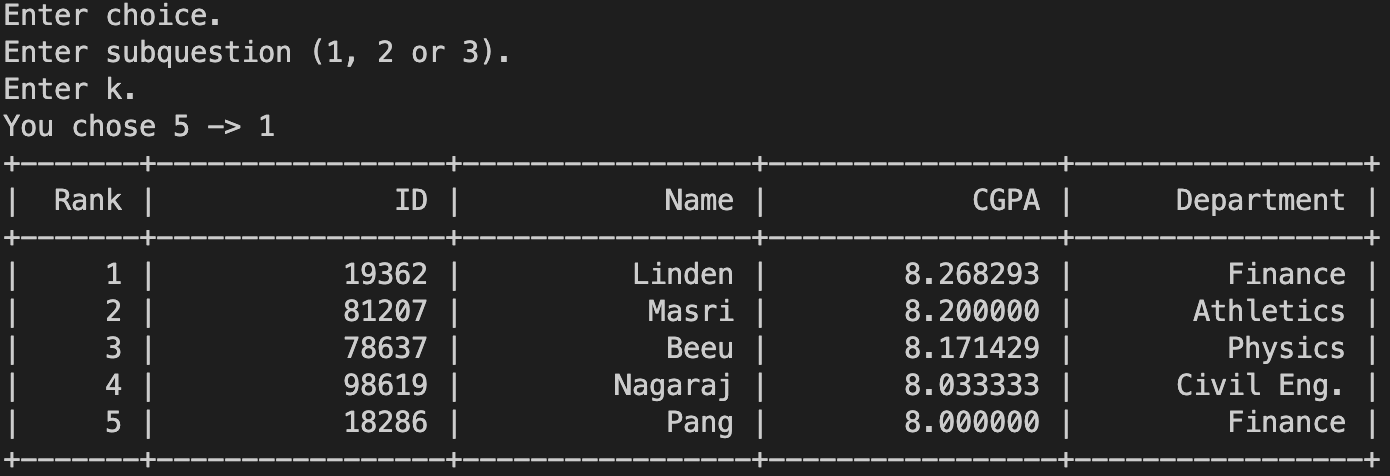
\includegraphics[scale = 0.5]{5_1.png}

    Subquestion 2: Print the top-5 students with highest CGPA  for departments: Psychology, Elec. Eng., and Civil Eng.


    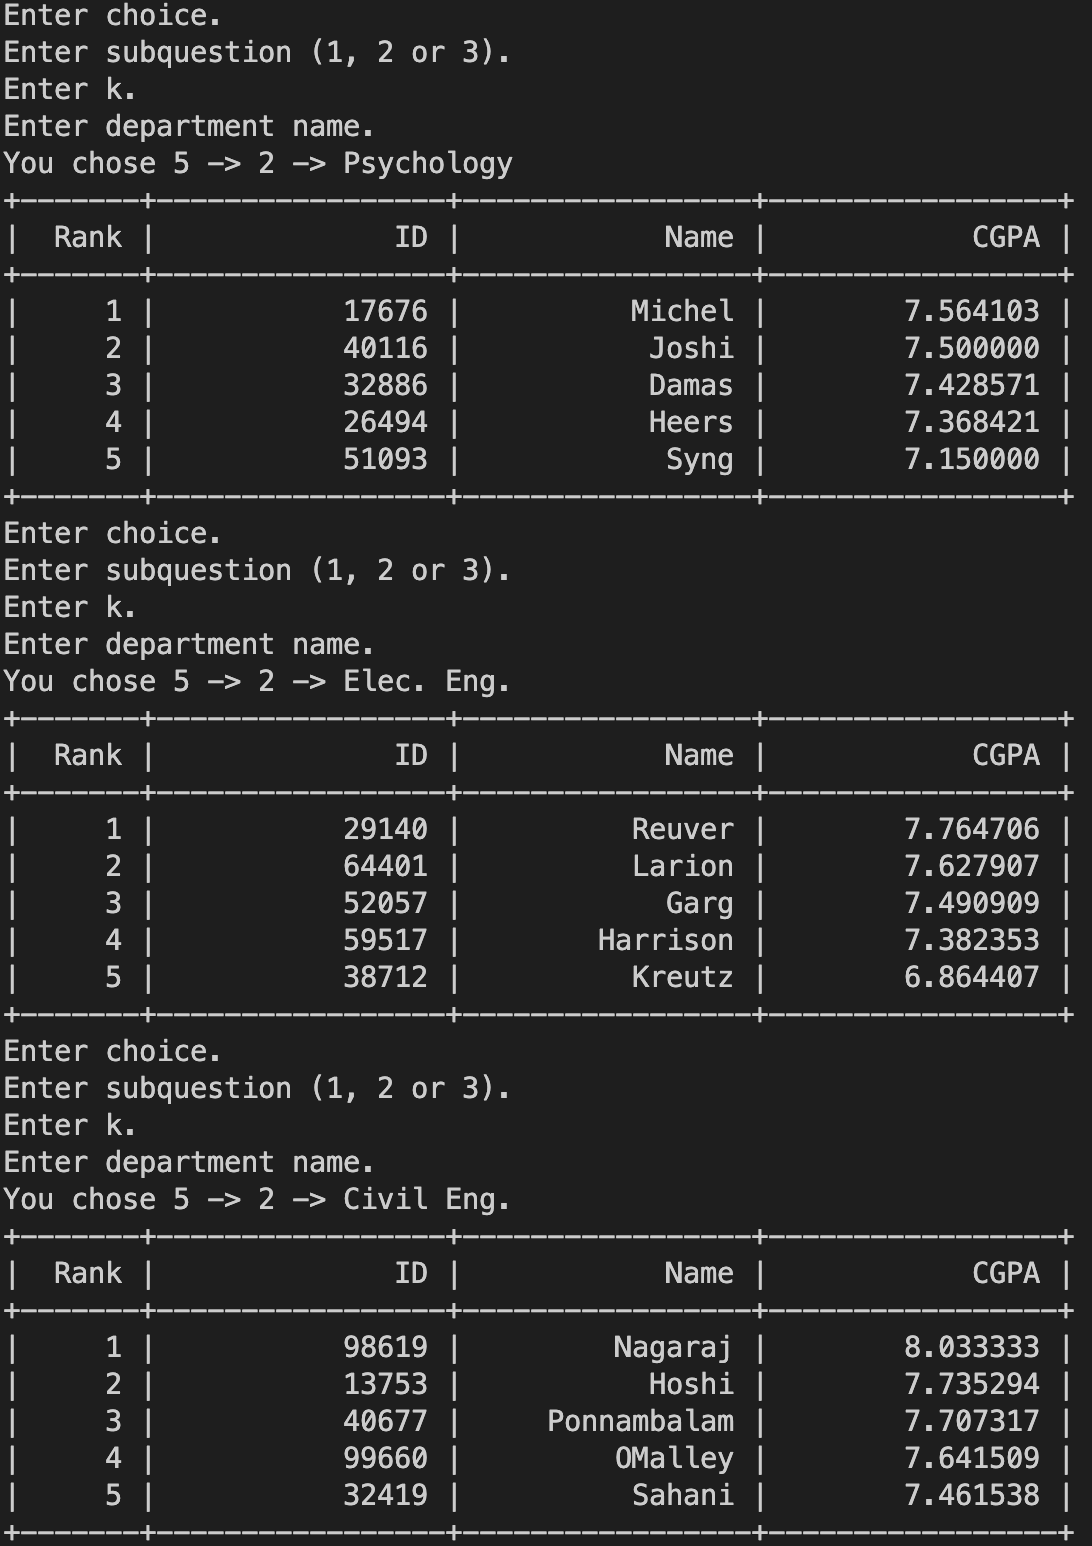
\includegraphics[scale = 0.5]{5_2.png}
\newpage
    Subquestion 3: Print the top-5 students with highest CGPA  for  course ids: 237, 349, 735

    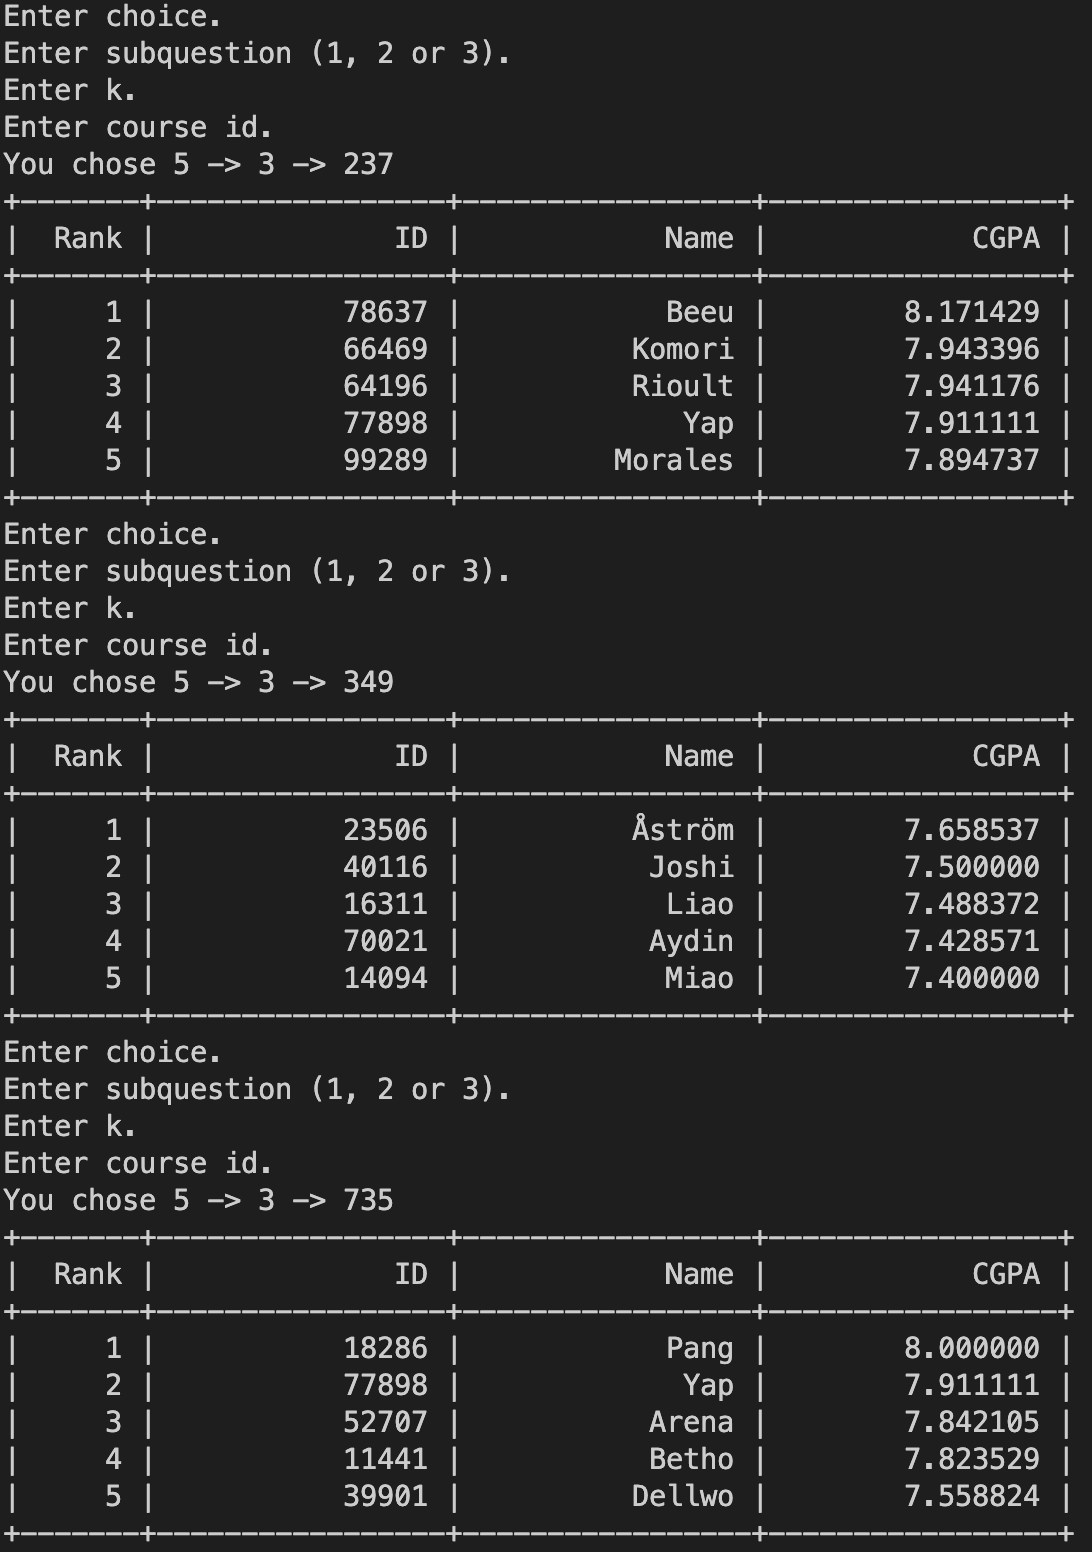
\includegraphics[scale = 0.5]{5_3.png}

\end{document}